%%%%%%%%%%%%%%%%%%%%%%%%%%%%%%%%%%%%%%%%%%%%%%%%%%%%%%%%%%%
%%%%%%%%%%%%%%%%%%%%%%%%%%%%%%%%%%%%%%%%%%%%%%%%%%%%%%%%%%%
\subsection{Material Scientific and Pre-optimization}
%\subsubsection{Solution}
%%%%%%%% AQUATIC 
As already indicated in the experimental section the aquatic recipe adopted from Anwar et al.\cite{Anwar2017} failed to produce a homogeneous layer. 
The solution was opaque from the beginning and the resulting layers were patchy and laced with cracks (see figure \ref{fig:sem-old}). 
Altering the ratios of ingredients, adjusting pH (by adding \gls{naoh}, \ch{H2SO4} or \gls{hcl}) or adding \gls{sds} as surfactant didn't improve the resulting \gls{zro} layers. 
% ../../Data/SEM/SEM_2020_11_10_Old_Recipes/10_2L_19.tif
% ../../Data/SEM/SEM_2020_11_19_Old_Recipes/71_SL_NT4_11.tif
Even after the consecutive application of two layers there was no clear improvement and the results reminded rather of a sparse crust than of a film. 
%It is assumed that the solution was far from the optimum for a sol-gel process. 
%
Figure \ref{fig:sem-old} shows a typical details of \gls{zro} (dark) on top of \gls{fto} (finely polycrystalline). 
%These were the results of a single (figure \ref{fig:sem-old1}) and double (figure \ref{fig:sem-old2}) "layer" of the aquatic recipe. 
Large cracks, non coated areas and inhomogeneity were 
%part of (ausmachen) 
shared characteristics among 
all samples created with the aquatic recipe. 
%even after several/multiple/various alteration to the recipe. 

The sol-gel recipe optimized by Hu et al.\cite{Hu2016} for \ch{Al2O3} worked splendidly for our use case even after (not so) minor changes (see section \ref{sec:exp-sol-bu}). 
%
Figure \ref{fig:sem-ph} shows a top view of 10 layers of the buthanolic solution on top of a steel substrate. 
%%%% PIN HOLES
The large irregularity on the bottom left could depict a pin hole, a (tiny) hole that reaches to the substrate. 
These irregularities are rather the exception. 
Alternatively, the small, hardly visible slits spread across the surface could depict such pin holes. 
These - I think - are rather only one layer deep irregularities since they are so prevalent
and hardly any pin holes were electrically observed on similar samples. 


%%%%%% STABILITY
As soon as the solution showed initial cloudiness, it was declared as unstable. 
The visually asserted stability of the solution could be increased a lot by replacing the stabilizing agent (\gls{acoh}) with \gls{ipo}.
A solution with \gls{acoh} was stable for approximately \td{24h} sealed with Parafilm. 
%192 was first with IPOH
Whereas a solution with \gls{ipo} as stabilizing agent stayed stable for circa \td{72h}. 
An increase of the \gls{zrpro} concentration accelerates the aging process of the solution.
%
Only the introduction of \gls{ipo} into the recipe allowed higher concentrated solutions to be practicable 
as they could be stored until the next time needed instead of producing a separate solution for each sample.
It was discovered that after a \gls{acoh} solution has aged beyond cloudiness 
the addition of a small amount of \gls{ipo} can even reversed the aging effect. % for \td{respectable} amount of time. 
This effect is not only due to dilution as additional solvent (\gls{buoh}) did not re-stabilize the solution, 
even after 5 fold dilution. 
%Whereas addition of the original stabilizing agent \gls{buoh} to an aged solution had no effect. 
%Whereas, when the addition of the original stabilizing agent \gls{buoh} to an aged solution had no effect. 

\begin{figure}[htb]
    \centering
    \begin{subfigure}{.45\textwidth}
        \centering
        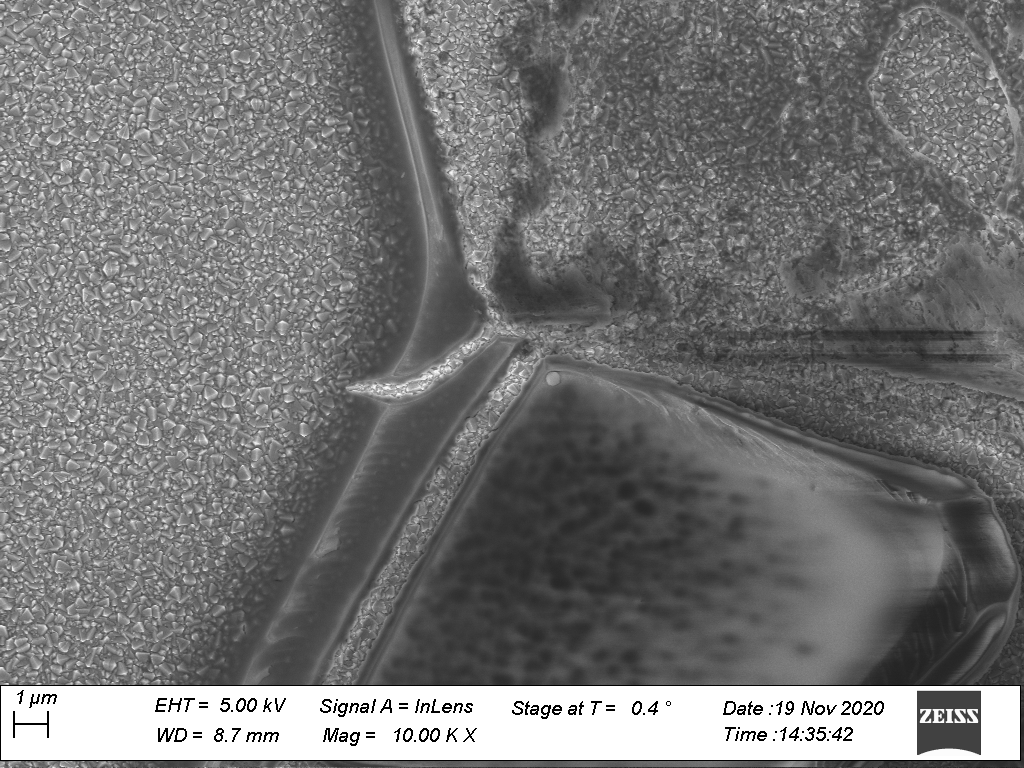
\includegraphics[width=.79\textwidth]{Pics/sem/071_fto_old_1x1F.png}
        \caption{SEM picture of \gls{zro} produces by H2O solution} \label{fig:sem-old}
    \end{subfigure}
    \begin{subfigure}{.45\textwidth}
        \centering
        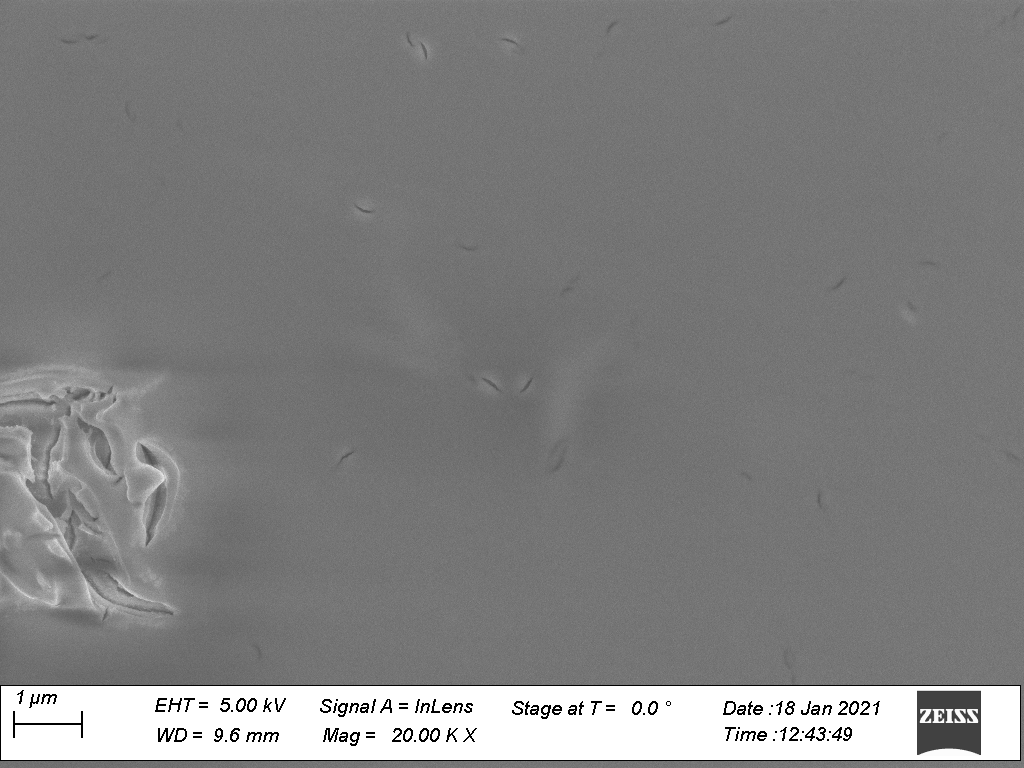
\includegraphics[width=.79\textwidth]{Pics/sem/147_steel_ph_10x.png}
        \caption{SEM picture of \gls{zro} produced by buoh solution} \label{fig:sem-ph}
    \end{subfigure}
    \begin{subfigure}{.45\textwidth}
        \centering
        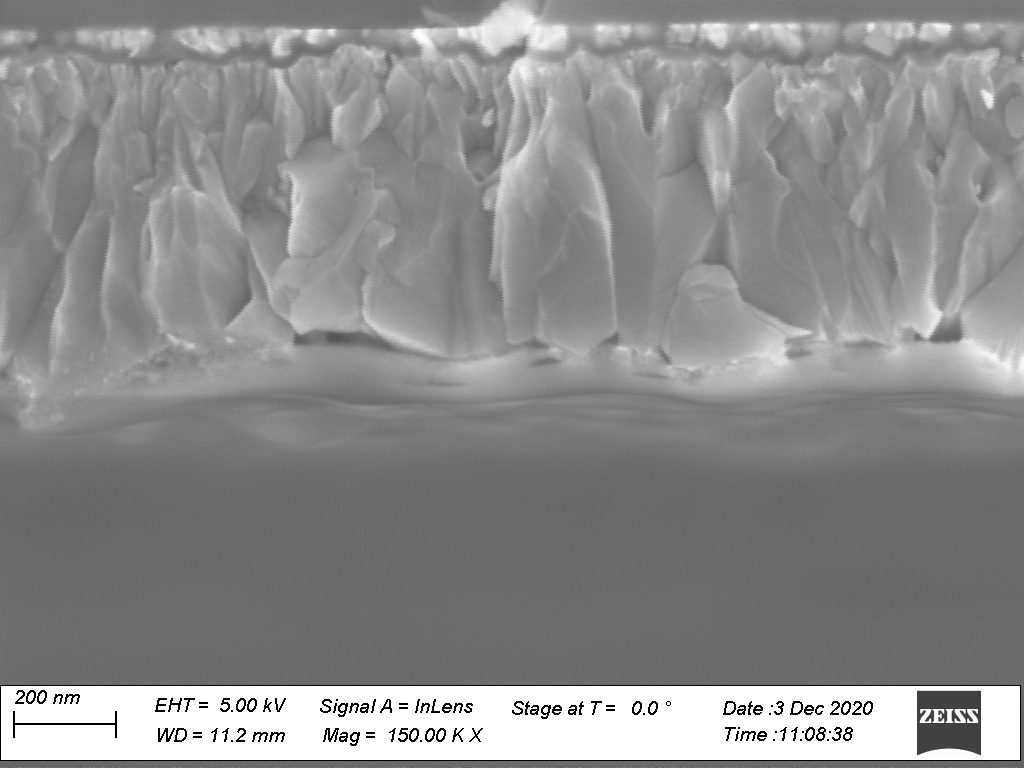
\includegraphics[width=.8\textwidth]{Pics/sem/115_fto_cs_1x.png}
        \caption{115 fto cs 1x} \label{fig:sem-cs1}
    \end{subfigure}
    \begin{subfigure}{.45\textwidth}
        \centering
        %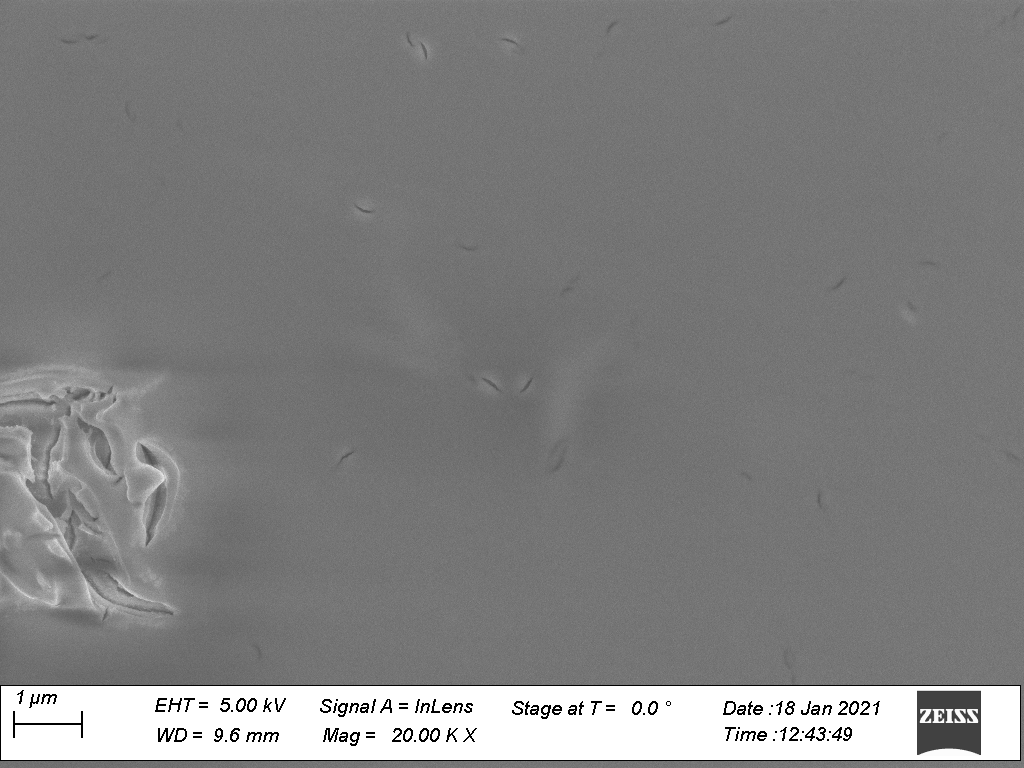
\includegraphics[width=.8\textwidth]{Pics/sem/147_steel_ph_10x.png}
        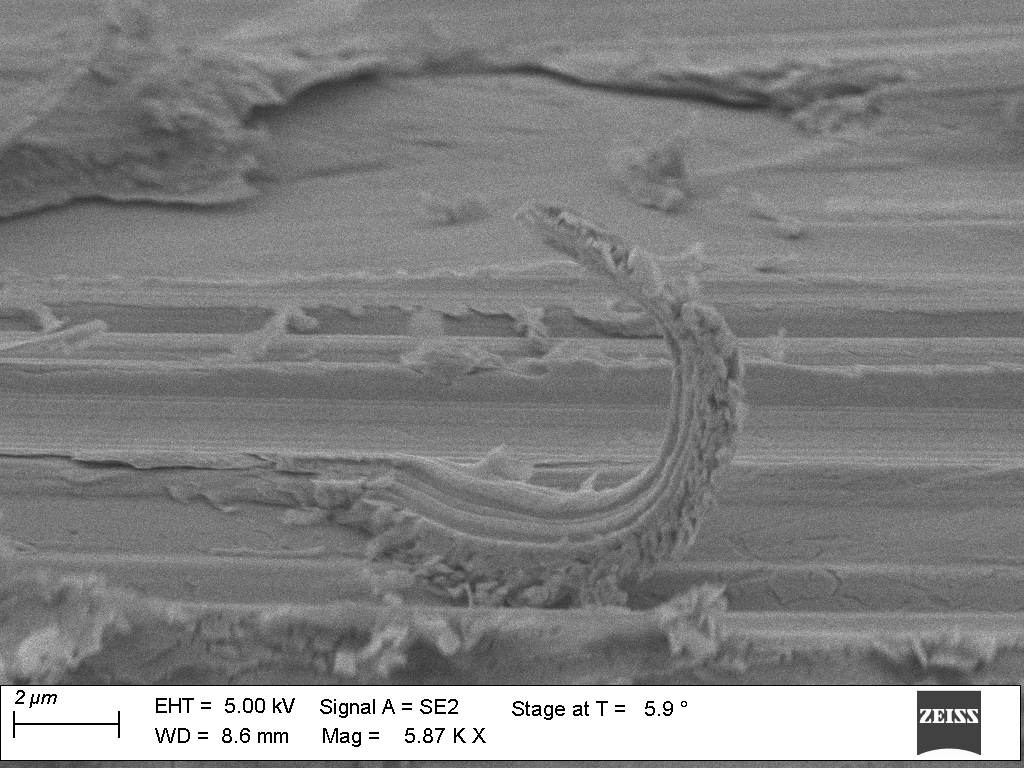
\includegraphics[width=.8\textwidth]{Pics/sem/150_steel_cs_2Fx5.png}
        \caption{150 steel 2Fx5} \label{fig:sem-cs2}
    \end{subfigure}
    \caption{SEM images of \gls{zro} on top of \gls{fto} (a,c) and \gls{zro} on steel (b,d)} \label{fig:sem}
\end{figure}


%%%%%%%%% CROSS SECTION
Figure \ref{fig:sem-cs1} shows the cross section of a single layer of \gls{zro} on \gls{fto} glass at a deliberate fracture.
The large crystalline part which makes up most of the image is \gls{fto}. 
The boundary to glass is visible at the very top. 
%On the lower edge of \gls{fto} a circa 100nm thick homogeneous layer can be observed: \gls{zro} produced by buthanolic recipe inspired by Hu et al..
On the lower edge of \gls{fto} a circa 100nm thick homogeneous layer of \gls{zro} (produced with buthanolic recipe)  can be observed.
%
Measuring the cross section on steel was not as straight forward because of the ductility of steel. 
The only way to get an insight into the thickness of the layer via \gls{sem} was through 
scratching the surface with an diamond glass cutter. 
The result can be seen in figure \ref{fig:sem-cs2}. 
5 layers of double concentrated solution were applied to this sample. 
Assuming that the raised structure resembling a tentacle is \gls{zro}, 
the thickness of the layer can be estimated to be around \um{1}.
%%%%%%%%%%%%%%%%%%%%%%%%%%%%%%%%%%%%%%%%%%%%%%%%%%%%%%%%%%%
%%%%%%%%%%%%%%%%%%%%%%%%%%%%%%%%%%%%%%%%%%%%%%%%%%%%%%%%%%%
%\subsubsection{SEM}

%The \gls{sem} pictures were not easy to take since 
%it has been tried to create an insulator 
%and the quality of the picture relies on the conductance of the material's surface. 
%This means that the better the quality of the resulting layer the more tedious it was to take a decent SEM image. 

%
%5F ca 100min
%4F ca 140min
%3F ca 420min (7h)
%extra AcOH stabilzed but needed so much that dilution too large...
%\td{IPO influence on "stability" p74: 600ul IPO makes clear, 4000 ul BuOH not clear with 
%same base solution (1ml of 4F), added extra 400ul to BuOH sol and after 5min clear. 
%of 1:5 is unacceptable Dilution }
%- 21.8 (1F) from 15.02. 13:30 bis 
%26.3 (1ml iPO to ca2ml of 5f) from 16.02. 16:30 bis 18.02.++
%18.02 4F in 80min milky
%      2F in ca 24h (stabilization AcOH)
%
%acceptable layer was produced by buthanolic solution, but very unstable (short lived) how long? p41 
%\Gls{ipo} solution allowed to even reuse high concentrated solution, which would otherwise become cloudy under 60 minutes. 
%Multiple question still need to be answered: 
%What causes the cloudiness (as stability increased through sealing probably \ch{H2O} from the air or \ch{O2}) and what's the mechanism? 
%How does \gls{ipo} increase the stability? 
%Does it do so because it "fits" better with the solvent. 
%As the original solvent was 2-methoxy-ethonanol instead of \ch{buoh}. 
%It was even observed that the addition of \td{some drops of} \gls{ipo} to an acetic solution can clear the solution.
%5F acetic solution milky over night 5:1 dilution with \gls{ipo} and clear after one minute of stirring and stayed clear over 5 nights.
% more details on pages 68ff
%No effect on the solution or the resulting layer was noticed \td{from the initial stirring}
%\todo{Following stirring times (in minutes) were tested and didn't have an influence on stability of the solution: 10-10-20, 10-10-45, 30-30-180.}
%The stirring time was untersucht, but not much difference so shortest was used because 
%short time can produces faster and the resulting solution is longer stable 
%(after finishing mixing)

%\td{instead of changing the stabilisation agent before optimisation, could change after pso, was vor und nachteile?}
%after realizing the improved effectiveness of \gls{ipo} for experimentation, 
%it was decided that EMMA will be executed with \gls{ipo} solution.


%- first recipe tried to improve to achieve more resisting layer. 
%by pH value, surface tension and solution ratios 
%(only 10\% change because it was assumed, that the recipe is good and should be improved, 
%but the recipe should be altered thoroughly. 
%two layers were also tried but didn't even pass the visual examination/test/inspection. 
%A curst was produced. 
%It is assumed 

%\iffalse
%\begin{figure}
%    \centering
%    \begin{subfigure}{.45\textwidth}
%        \centering
%        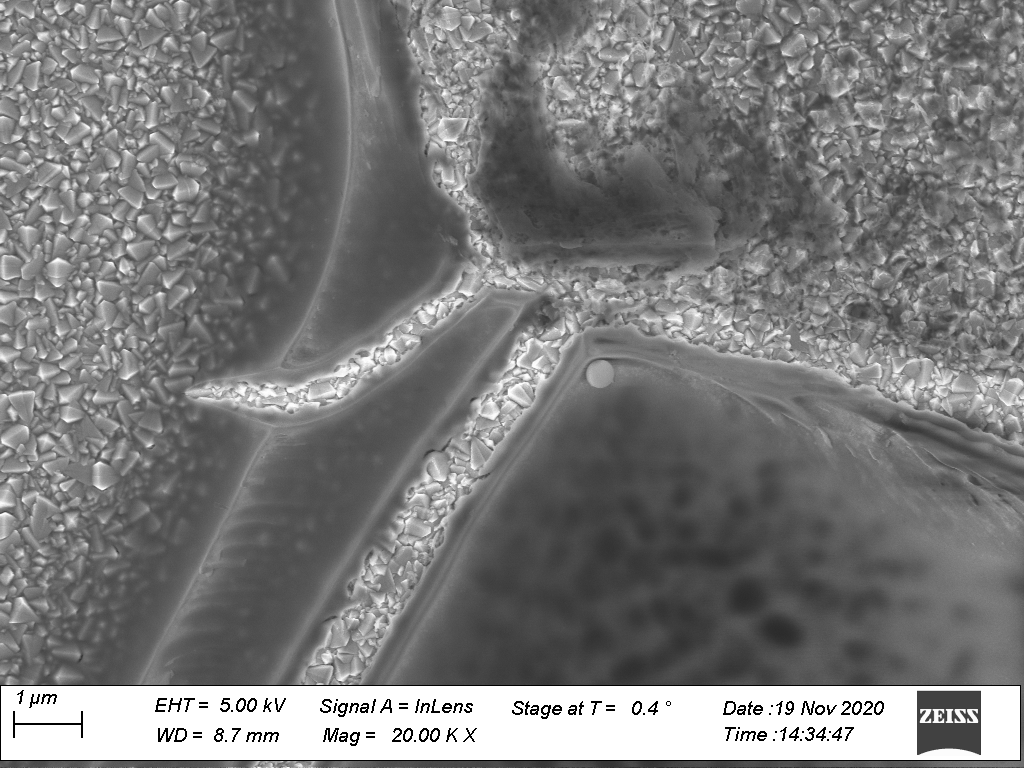
\includegraphics[width=.8\textwidth]{Pics/sem/071_fto_old_1x.png}
%        \caption{71 fto old 1x} \label{fig:sem-old1}
%    \end{subfigure}
%    \begin{subfigure}{.45\textwidth}
%        \centering
%        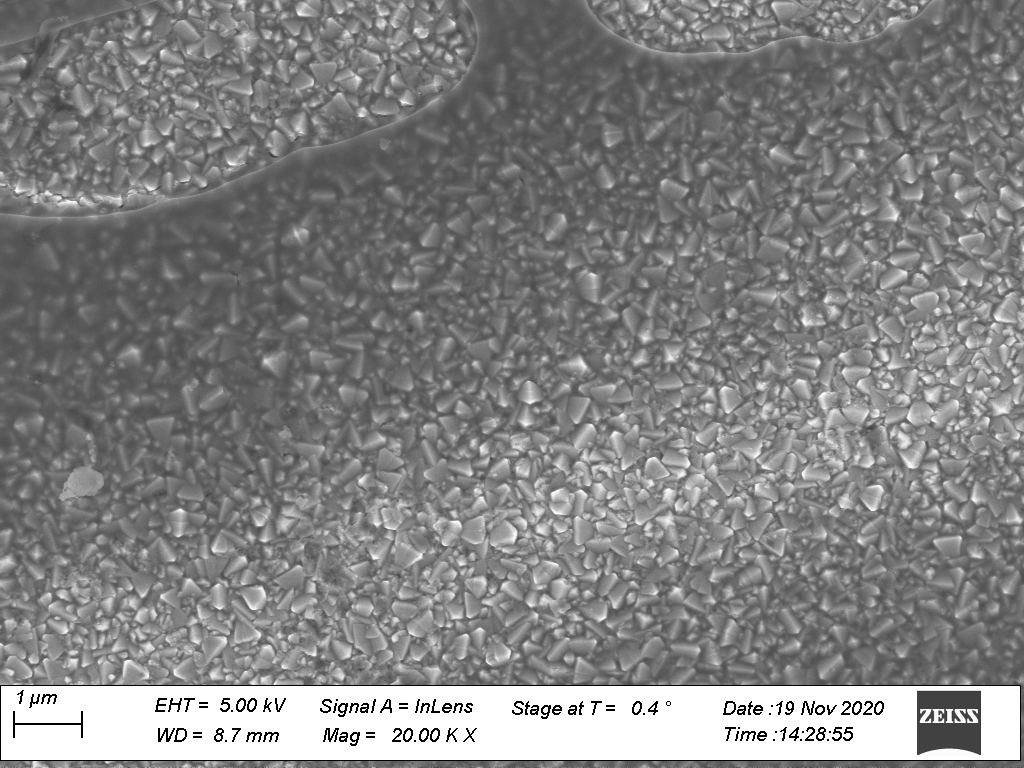
\includegraphics[width=.8\textwidth]{Pics/sem/071_fto_old_2x.png}
%        \caption{71 fto old 2x} \label{fig:sem-old2}
%    \end{subfigure}
%    \begin{subfigure}{.45\textwidth}
%        \centering
%        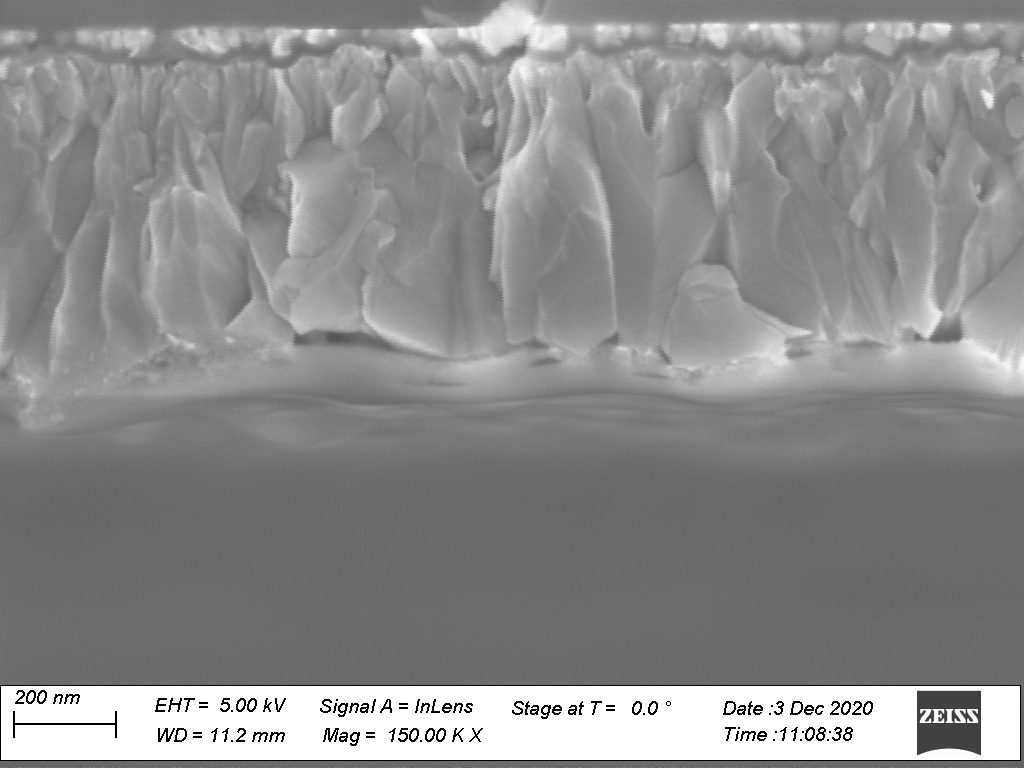
\includegraphics[width=.8\textwidth]{Pics/sem/115_fto_cs_1x.png}
%        \caption{115 fto cs 1x} \label{fig:sem-cs1}
%    \end{subfigure}
%    \begin{subfigure}{.45\textwidth}
%        \centering
%        %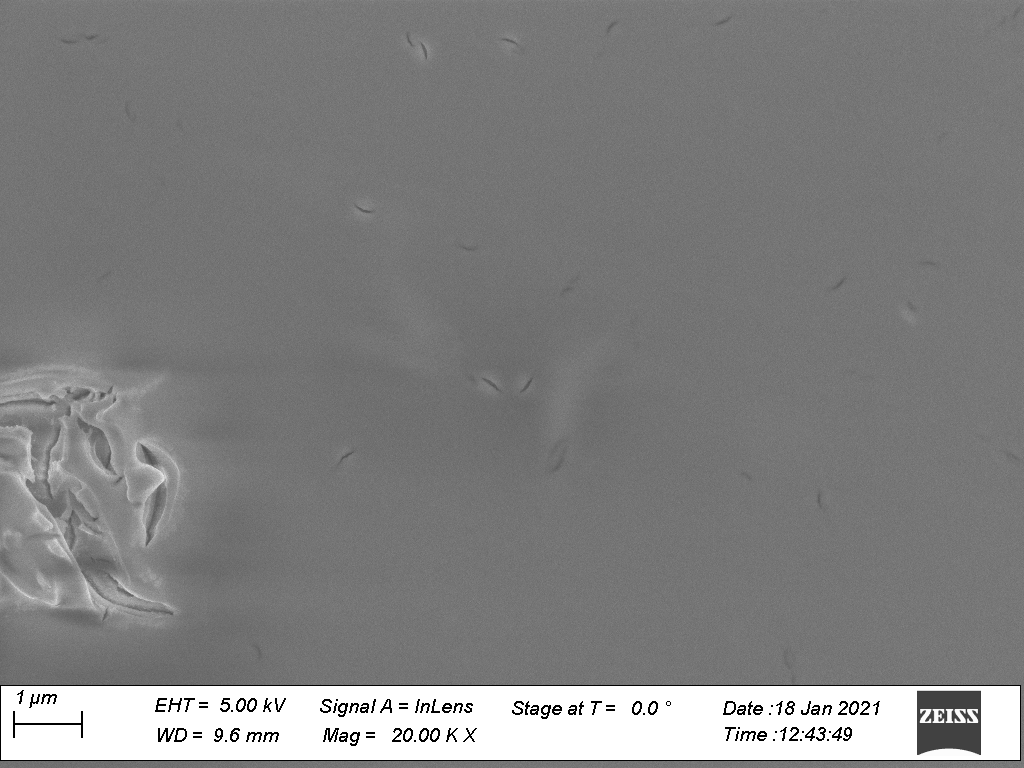
\includegraphics[width=.8\textwidth]{Pics/sem/147_steel_ph_10x.png}
%        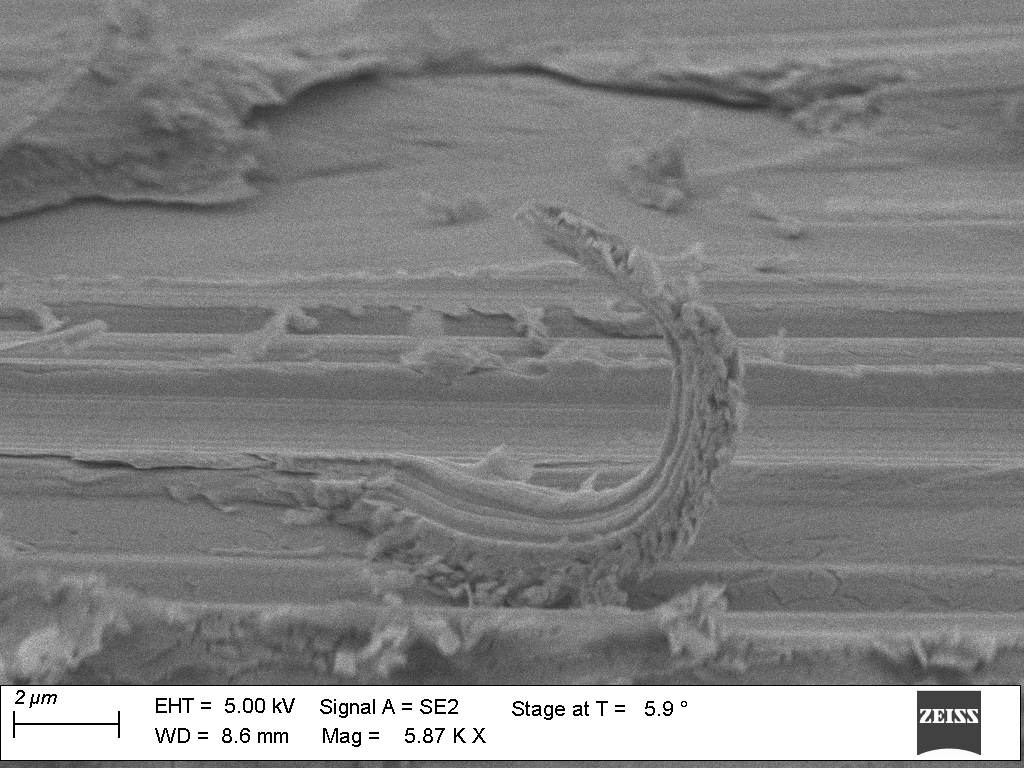
\includegraphics[width=.8\textwidth]{Pics/sem/150_steel_cs_2Fx5.png}
%        \caption{150 steel 2Fx5} \label{fig:sem-cs2}
%    \end{subfigure}
%    \caption{cross section}
%    \label{fig:sem}
%\end{figure}
%\fi


%\iffalse
%%%%%%%%%%%%%%%%%%%%%%%%%%%%%%%%%%%%%%%%%%%%%%%%%%%%%%%%%%%
%%%%%%%%%%%%%%%%%%%%%%%%%%%%%%%%%%%%%%%%%%%%%%%%%%%%%%%%%%%
\subsubsection{Infra Red}

\begin{figure}[htb]
    \centering
    \begin{subfigure}{.49\textwidth}
        \centering
        \includegraphics[width=.99\textwidth]{Pics/ir-gt.png}
        \caption{Transmittance of \gls{zro} on glass} \label{fig:ir-gt}
    \end{subfigure}
    \begin{subfigure}{.49\textwidth}
        \centering
        \includegraphics[width=.99\textwidth]{Pics/ir-gr.png}
        \caption{reflectance of \gls{zro} on glass} \label{fig:ir-gr}
    \end{subfigure}
    \caption{IR} \label{fig:ir}
\end{figure}

In figure \ref{fig:ir-gt} transmission spectra of visible and \gls{nir} light can be seen. 
Each sample had different numbers of layers. 
The incident angle was 0 degree for each sample.
%differnt numbers of layers of \gls{zro} on a glass slide with 0 degree incident angle. 
The more layers the more of the light is absorbed (1000nm) by the \gls{zro} layers. 
%The trend is not monotonic due to inhomogenities in the sample???b
The thicker the layer is the more wavy the graph, which most likely can be attributed to interference.
This trend can also be observed in figure \ref{fig:ir-gr}.
The light interference patterns at low wavelengths indicate that the thickness of the film is in the order of magnitude of the wavelengths\cite{delimafilho2017film}. 
Figure \ref{fig:ir-gr} shows reflectance spectra of visible and \gls{nir} at an incident angle of 45 degrees. 
The shift of the wavy part of the spectra (comparing reflectance with transmittance) 
can be explained by the longer path of light through the \gls{zro} layer because of the incident angle. 
%\fi

%%%%%%%%%%%%%%%%%%%%%%%%%%%%%%%%%%%%%%%%%%%%%%%%%%%%%%%%%%%
%%%%%%%%%%%%%%%%%%%%%%%%%%%%%%%%%%%%%%%%%%%%%%%%%%%%%%%%%%%
\subsubsection{Current Voltage Curves} 
\begin{figure}
    \centering
    \begin{subfigure}{.3\textwidth}
        \includegraphics[width=\textwidth]{Pics/iv/log-154-good-3x4F.png}
        \caption{log good 3x4F} \label{fig:iv-log-good}
    \end{subfigure}
    \begin{subfigure}{.3\textwidth}
        \includegraphics[width=\textwidth]{Pics/iv/log-146-okay-10x1F.png}
        \caption{log okay 10x1F} \label{fig:iv-log-okay}
    \end{subfigure}
    \begin{subfigure}{.3\textwidth}
        \includegraphics[width=\textwidth]{Pics/iv/log-156-bad-3x3F.png}
        \caption{log bad 3x3F} \label{fig:iv-log-bad}
    \end{subfigure}
    \begin{subfigure}{.3\textwidth}
        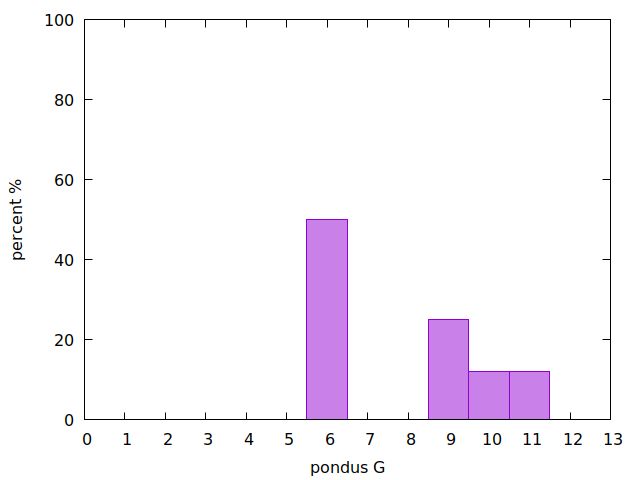
\includegraphics[width=\textwidth]{Pics/iv/stat-154-okay-3x4F.png}
        \caption{stat good 3x4F} \label{fig:iv-stat-good}
    \end{subfigure}
    \begin{subfigure}{.3\textwidth}
        \includegraphics[width=\textwidth]{Pics/iv/stat-146-good-10x1F.png}
        \caption{stat okay 10x1F} \label{fig:iv-stat-okay}
    \end{subfigure}
    \begin{subfigure}{.3\textwidth}
        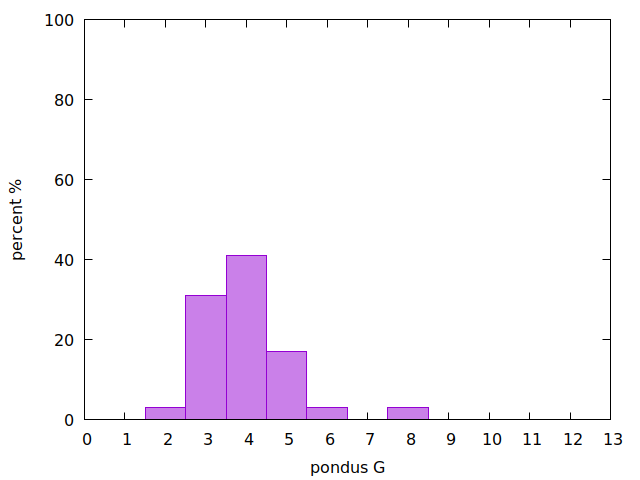
\includegraphics[width=\textwidth]{Pics/iv/stat-156-bad-3x3F.png}
        \caption{stat bad 3x3F} \label{fig:iv-stat-bad}
    \end{subfigure}
    \caption{maybe remove 146 and make 154 good AND set yrange [E-1:E-14] and show phd threshold} \label{fig:iv}
\end{figure}

%Figures \ref{fig:iv-log-good} and \ref{fig:iv-stat-good} are measurements from a good sample. 
Figure \ref{fig:iv-log-good} shows \gls{iv} curves in logarithmic scale of a insulating sample. 
Each line represents a I-V measurement at a distinct contact applied by sputtering through a mask. 
All of the curves show a max voltage of under \num{e-6} \SI{}{\volt} 
and quite a few show hardly any current which is the ideal. 
For each measurement the conductivity (i.e. the gradient at V=0) was calculated (see section \ref{sec:exp-eval}). 
Figure \ref{fig:iv-stat-good} shows the distribution of gradients for the same sample as in \ref{fig:iv-log-good}.
%
Figures \ref{fig:iv-log-okay} and \ref{fig:iv-stat-okay} show measurements from moderate sample. 
Most of the \gls{iv}s have a maximum voltage of under \num{e-6} V, 
but there are some so called pin holes with conductance above this threshold. %\num{e-6} V. 
%
In figures \ref{fig:iv-log-good} and \ref{fig:iv-log-okay} the minimum of the functions 
is not at \SI{0}{\volt}, which means that the function does not cross the origin. 
This deviation is similar to the deviation because of the photo-currents\cite{perez2018solar}, 
but was not investigated further. 
Though, the photo-current is compelling, it is most likely not zutreffend because of \gls{zro}'s band gap of \ev{5}\cite{sinhamahapatra2016oxygen}.
%
Finally, figures \ref{fig:iv-log-bad} and \ref{fig:iv-stat-bad} show a sample 
where all measurement exhibit relatively high voltages and high calculated conductances. 
This indicates a overall bad condition of the \gls{zro} layer for insulating. 

%%%%%%%%%%%%%%%%%%%%%%%%%%%%%%%%%%%%%%%%%%%%%%%%%%%%%%%%%%%
%%%%%%%%%%%%%%%%%%%%%%%%%%%%%%%%%%%%%%%%%%%%%%%%%%%%%%%%%%%
\subsubsection{XRD}
\begin{figure}
	\centering
	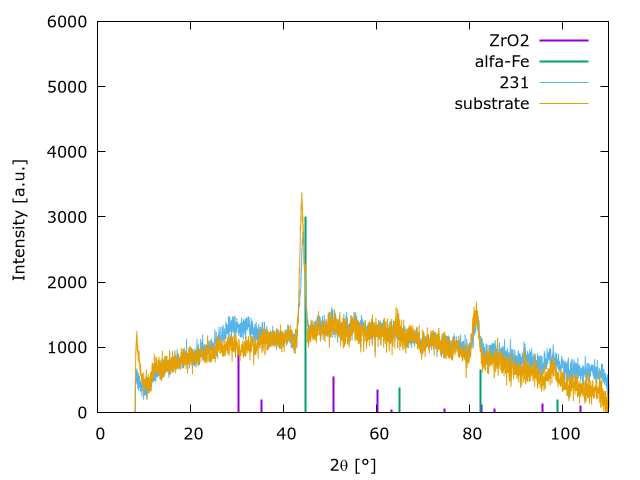
\includegraphics[width=\picwidth]{Pics/xrd.png}
	\caption{XRD spectra}
	\label{fig:xrd}
\end{figure}

Figure \ref{fig:xrd} shows \gls{xrd} spectra of the substrate, steel, and 
the substrate with ten layers of double concentrated solution (experiment number 6113, see \td{appendix}).
In addition two idealized spectra from the Crystallography Open Database of cubic \gls{zro} (COD ID 1521753\cite{gkatz1971xray}) and of $\alpha$-Fe (COD ID 1100108).
The four largest peaks of cubic \gls{zro} at $\theta=30, 51, 60, 35$ clearly stand out against the noise from the experimental spectrum. %can be clearly seen in the experimental spectra.
%In figure \ref{fig:xrd} the two strongest $\alpha$-Fe peaks can be seen clearly. 
%The highest peak of \gls{zro} is very \td{broadened} and is therefore not as distinct. 
%This wideness is is due to polycrystalline form of the material which is expected 
%due to the sol-gel creation process and multiple applications of layers. 
%Nonetheless, the \gls{xrd} spectra shows clearly that the produced layer is \gls{zro}.

%%%%%%%%%%%%%%%%%%%%%%%%%%%%%%%%%%%%%%%%%%%%%%%%%%%%%%%%%%%
%%%%%%%%%%%%%%%%%%%%%%%%%%%%%%%%%%%%%%%%%%%%%%%%%%%%%%%%%%%
\subsubsection{Preoptimization}
Before the optimization with the \gls{emma} algorithm, 
the boundaries of the input variables were explored. 
Especially, the \gls{db} velocity (i.e. the velocity with which the blade moves and spreads the solution over the sample)
was varied and examined during pre-optimization. 
The slower the \gls{db} velocity, the more uniformly the solution evaporated. 
If the \gls{db} velocity was too slow (less than \mmps{1}), no layer was formed. 
With the reason that the force exerted by the blade on the liquid not being strong enough to overcome surface tension. 
This means that behind the blade a meniscus would pull the liquid without leaving any for the gelling process. 
Additionally, the temperature while \gls{db} affects the resulting layer together with the \gls{db} velocity. 

%\td{Assumption: Ideally solution evaporate shortly after DB but not before}
%due to the boiling point of \gls{buoh} at 117 C\cite{ncbi1butanol} the room temperature to 80 C were used as temperature during \gls{db}.
%- p76, 146 (10x1F) good, 154 (3x4F) okay, 156 (3x3F) bad visualisation

